\section[Stress/Strain]{Stress/Strain plots}

\graphicspath{{Chapter5/Figs/}}

% //////////////////////////////////////////////////////////////////////////////
\begin{frame}
  \frametitle{Stress/Strain plots}
  \framesubtitle{}
  \label{ch5fr:stroptions}
\begin{scriptsize}


\emph{Plot stress}

\begin{itemize}
\item
  \texttt{-cstress}: Plot Coulomb Stress change.
\item
  \texttt{-sstress}: Plot Shear Stress change.
\item
  \texttt{-nstress}: Plot Normal Stress change.
\item
  \texttt{-fcross}: Plot cross section of stress change or dilatation.
\end{itemize}

\emph{Plot Strain components}

\begin{itemize}
\item
  \texttt{-stre**}: Where \texttt{**} you can fill all strain components
  \texttt{xx},\texttt{yy},\texttt{zz}, \texttt{yz}, \texttt{xz},
  \texttt{xy}.
\item
  \texttt{-strdil}: Plot dilatation (Exx + Eyy + Ezz )
\end{itemize}

\emph{Overlay Stress/strain on the top of DEM}

\texttt{-****+ot}: use \texttt{+ot} after the main argument to overlay
the raster output on the top of DEM. configure transparency in
\texttt{default-param} file. \textbf{Be careful} transparency can
printed only in JPEG, PNG and PDF outputs.
\end{scriptsize}
\end{frame}
\note{}

% //////////////////////////////////////////////////////////////////////////////
\begin{frame}[t,fragile]
  \frametitle{Coulomb Stress Change}
  \framesubtitle{Example 501}
  \label{ch5fr:ex501}
\begin{columns}[t]
  \begin{column}{.5\textwidth}
\begin{scriptsize}
\begin{verbatim}
$ ./coulomb2gmt.sh kef_1953 kef_1953_kef \
                   -outjpg \ 
                   --output example501 \
                   --logo_gmt \
                   --moment_tensor historic.cmt \
                   -fproj \
                   -fsurf \
                   -fdep \
                   -cstress
\end{verbatim}
\end{scriptsize}

  \end{column}
  \begin{column}{.5\textwidth}

\centering
  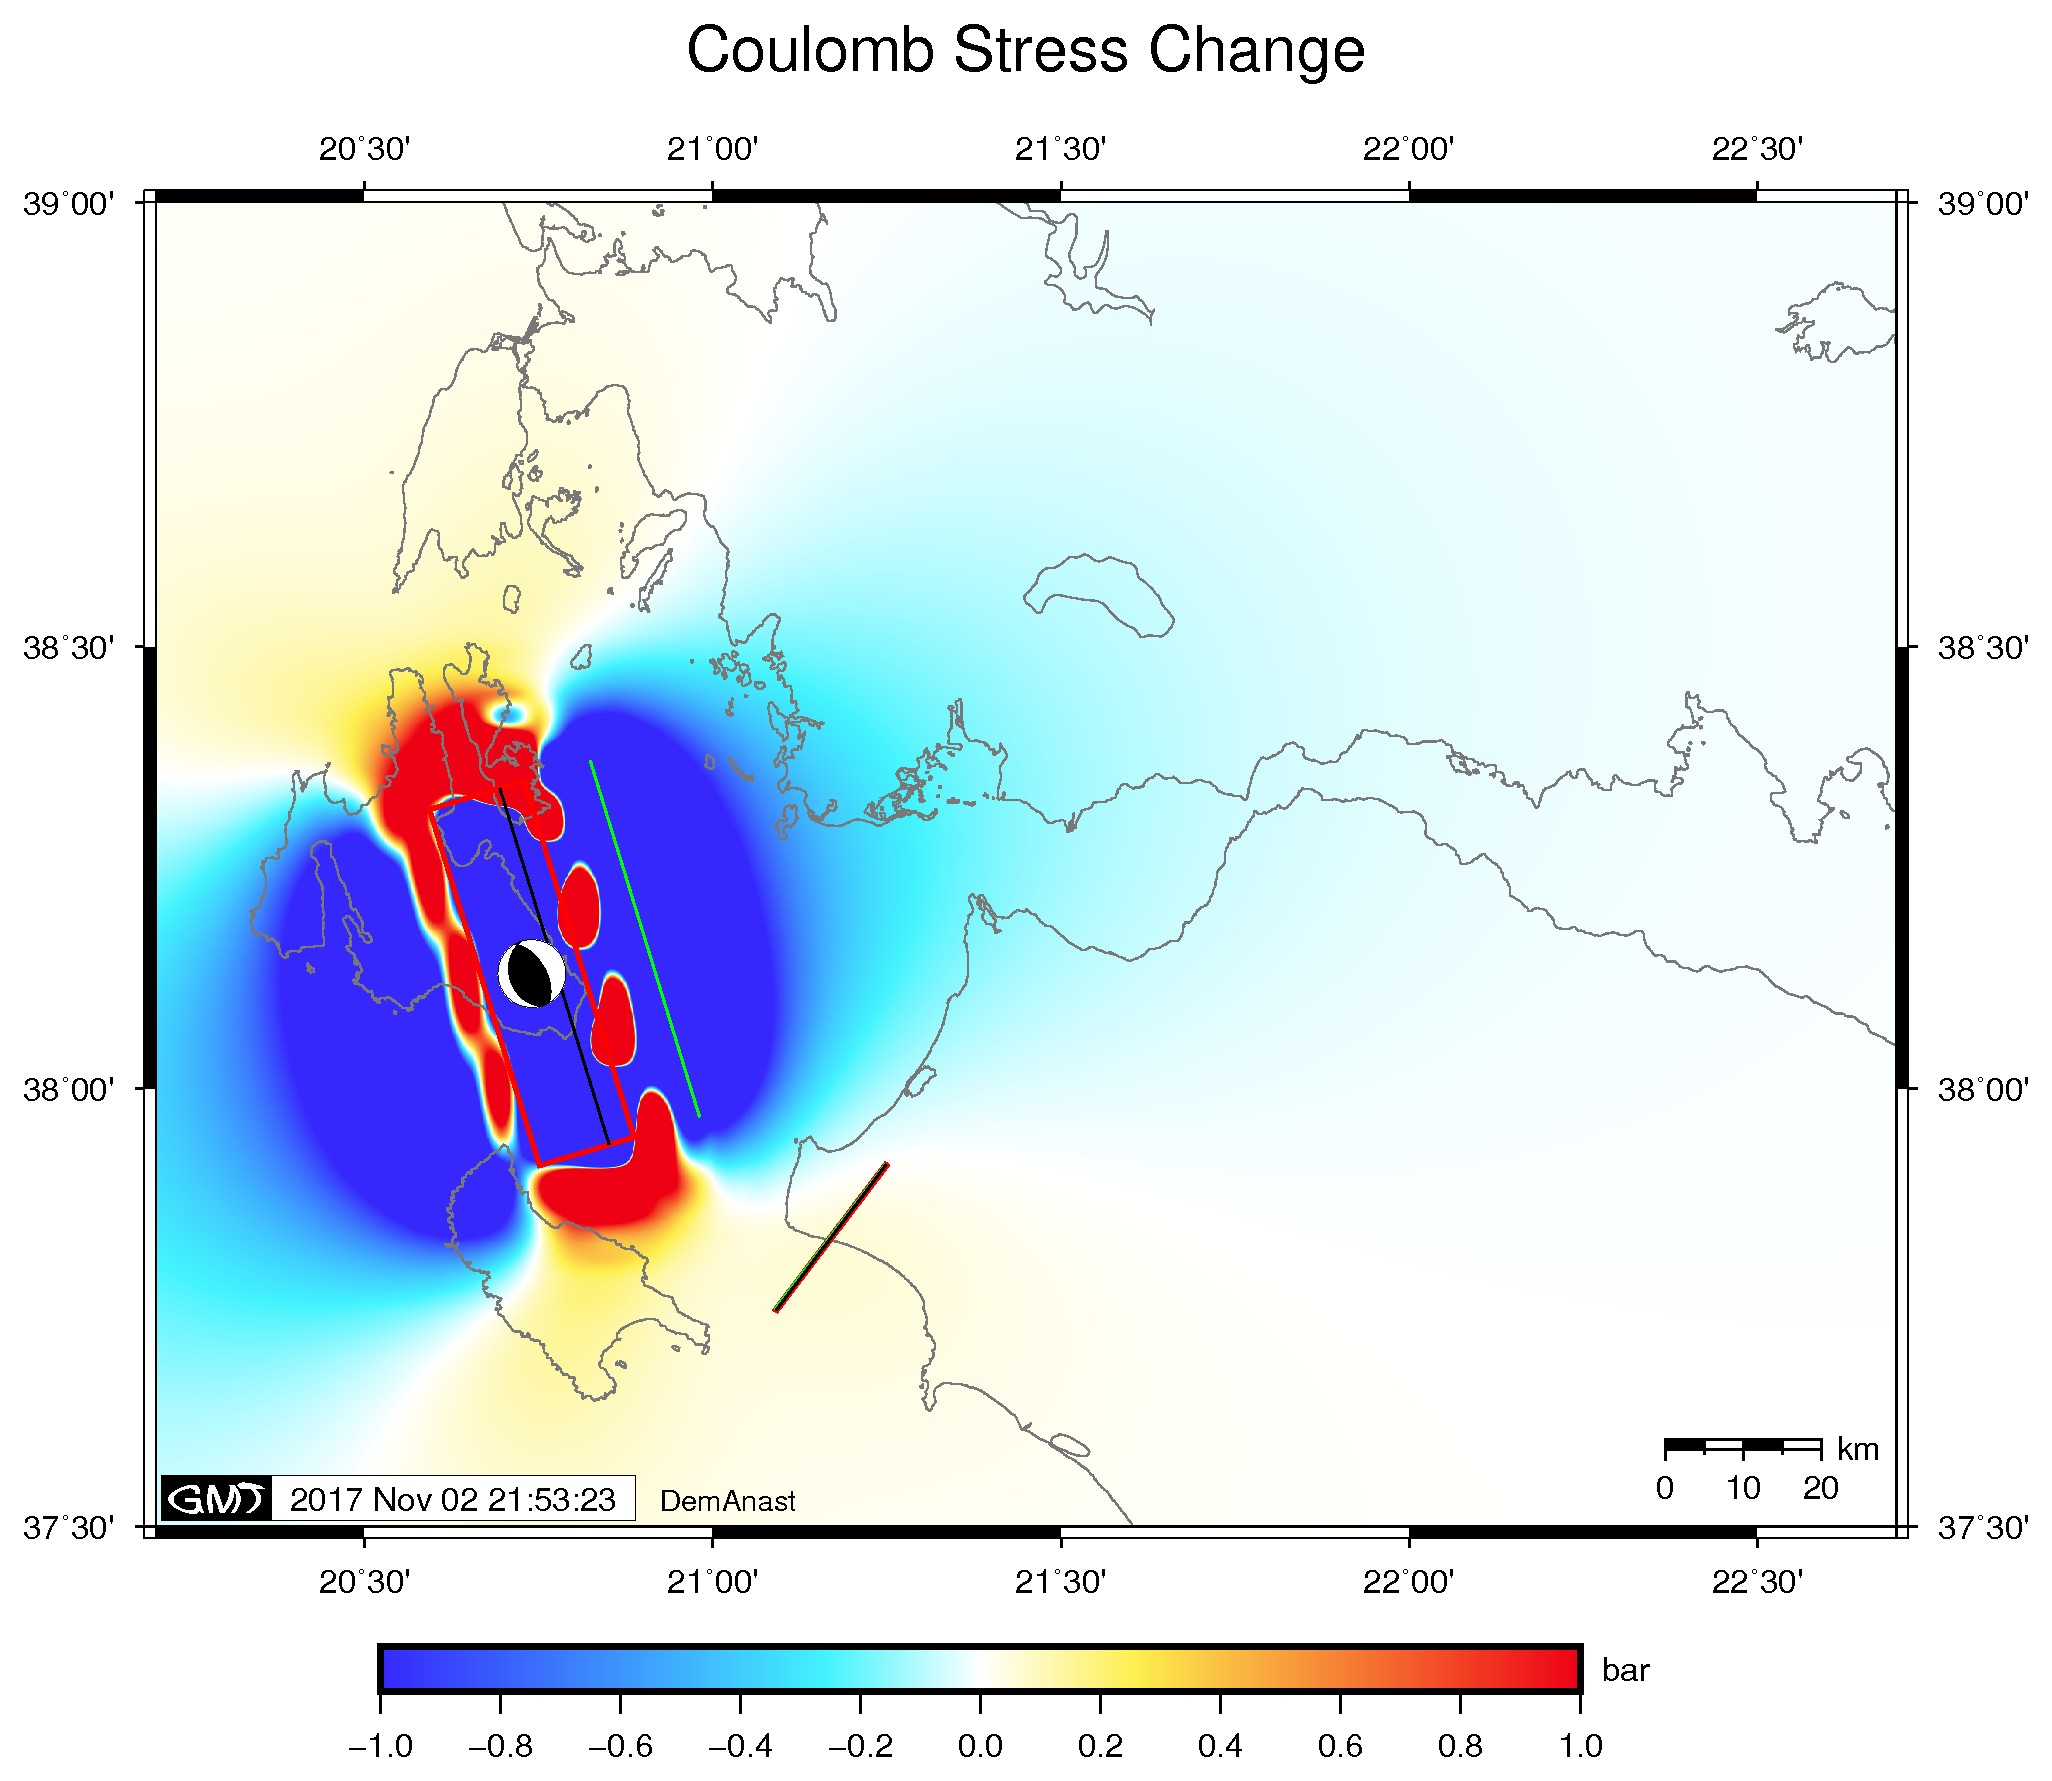
\includegraphics[width=.95\linewidth]{example501.jpg}
  \end{column}
\end{columns}

\end{frame}
\note{}

% //////////////////////////////////////////////////////////////////////////////
\begin{frame}[t,fragile]
  \frametitle{Coulomb Stress Change overlay topography}
  \framesubtitle{Example 502}
  \label{ch5fr:ex502}
\begin{columns}[t]
  \begin{column}{.5\textwidth}
\begin{scriptsize}
\begin{verbatim}
$ ./coulomb2gmt.sh kef_1953 kef_1953_kef \
                   -outjpg \ 
                   --output example502 \
                   --logo_gmt \
                   --moment_tensor historic.cmt \
                   -fproj \
                   -fsurf \
                   -fdep \
                   -cstress+ot
\end{verbatim}
\end{scriptsize}

  \end{column}
  \begin{column}{.5\textwidth}

\centering
  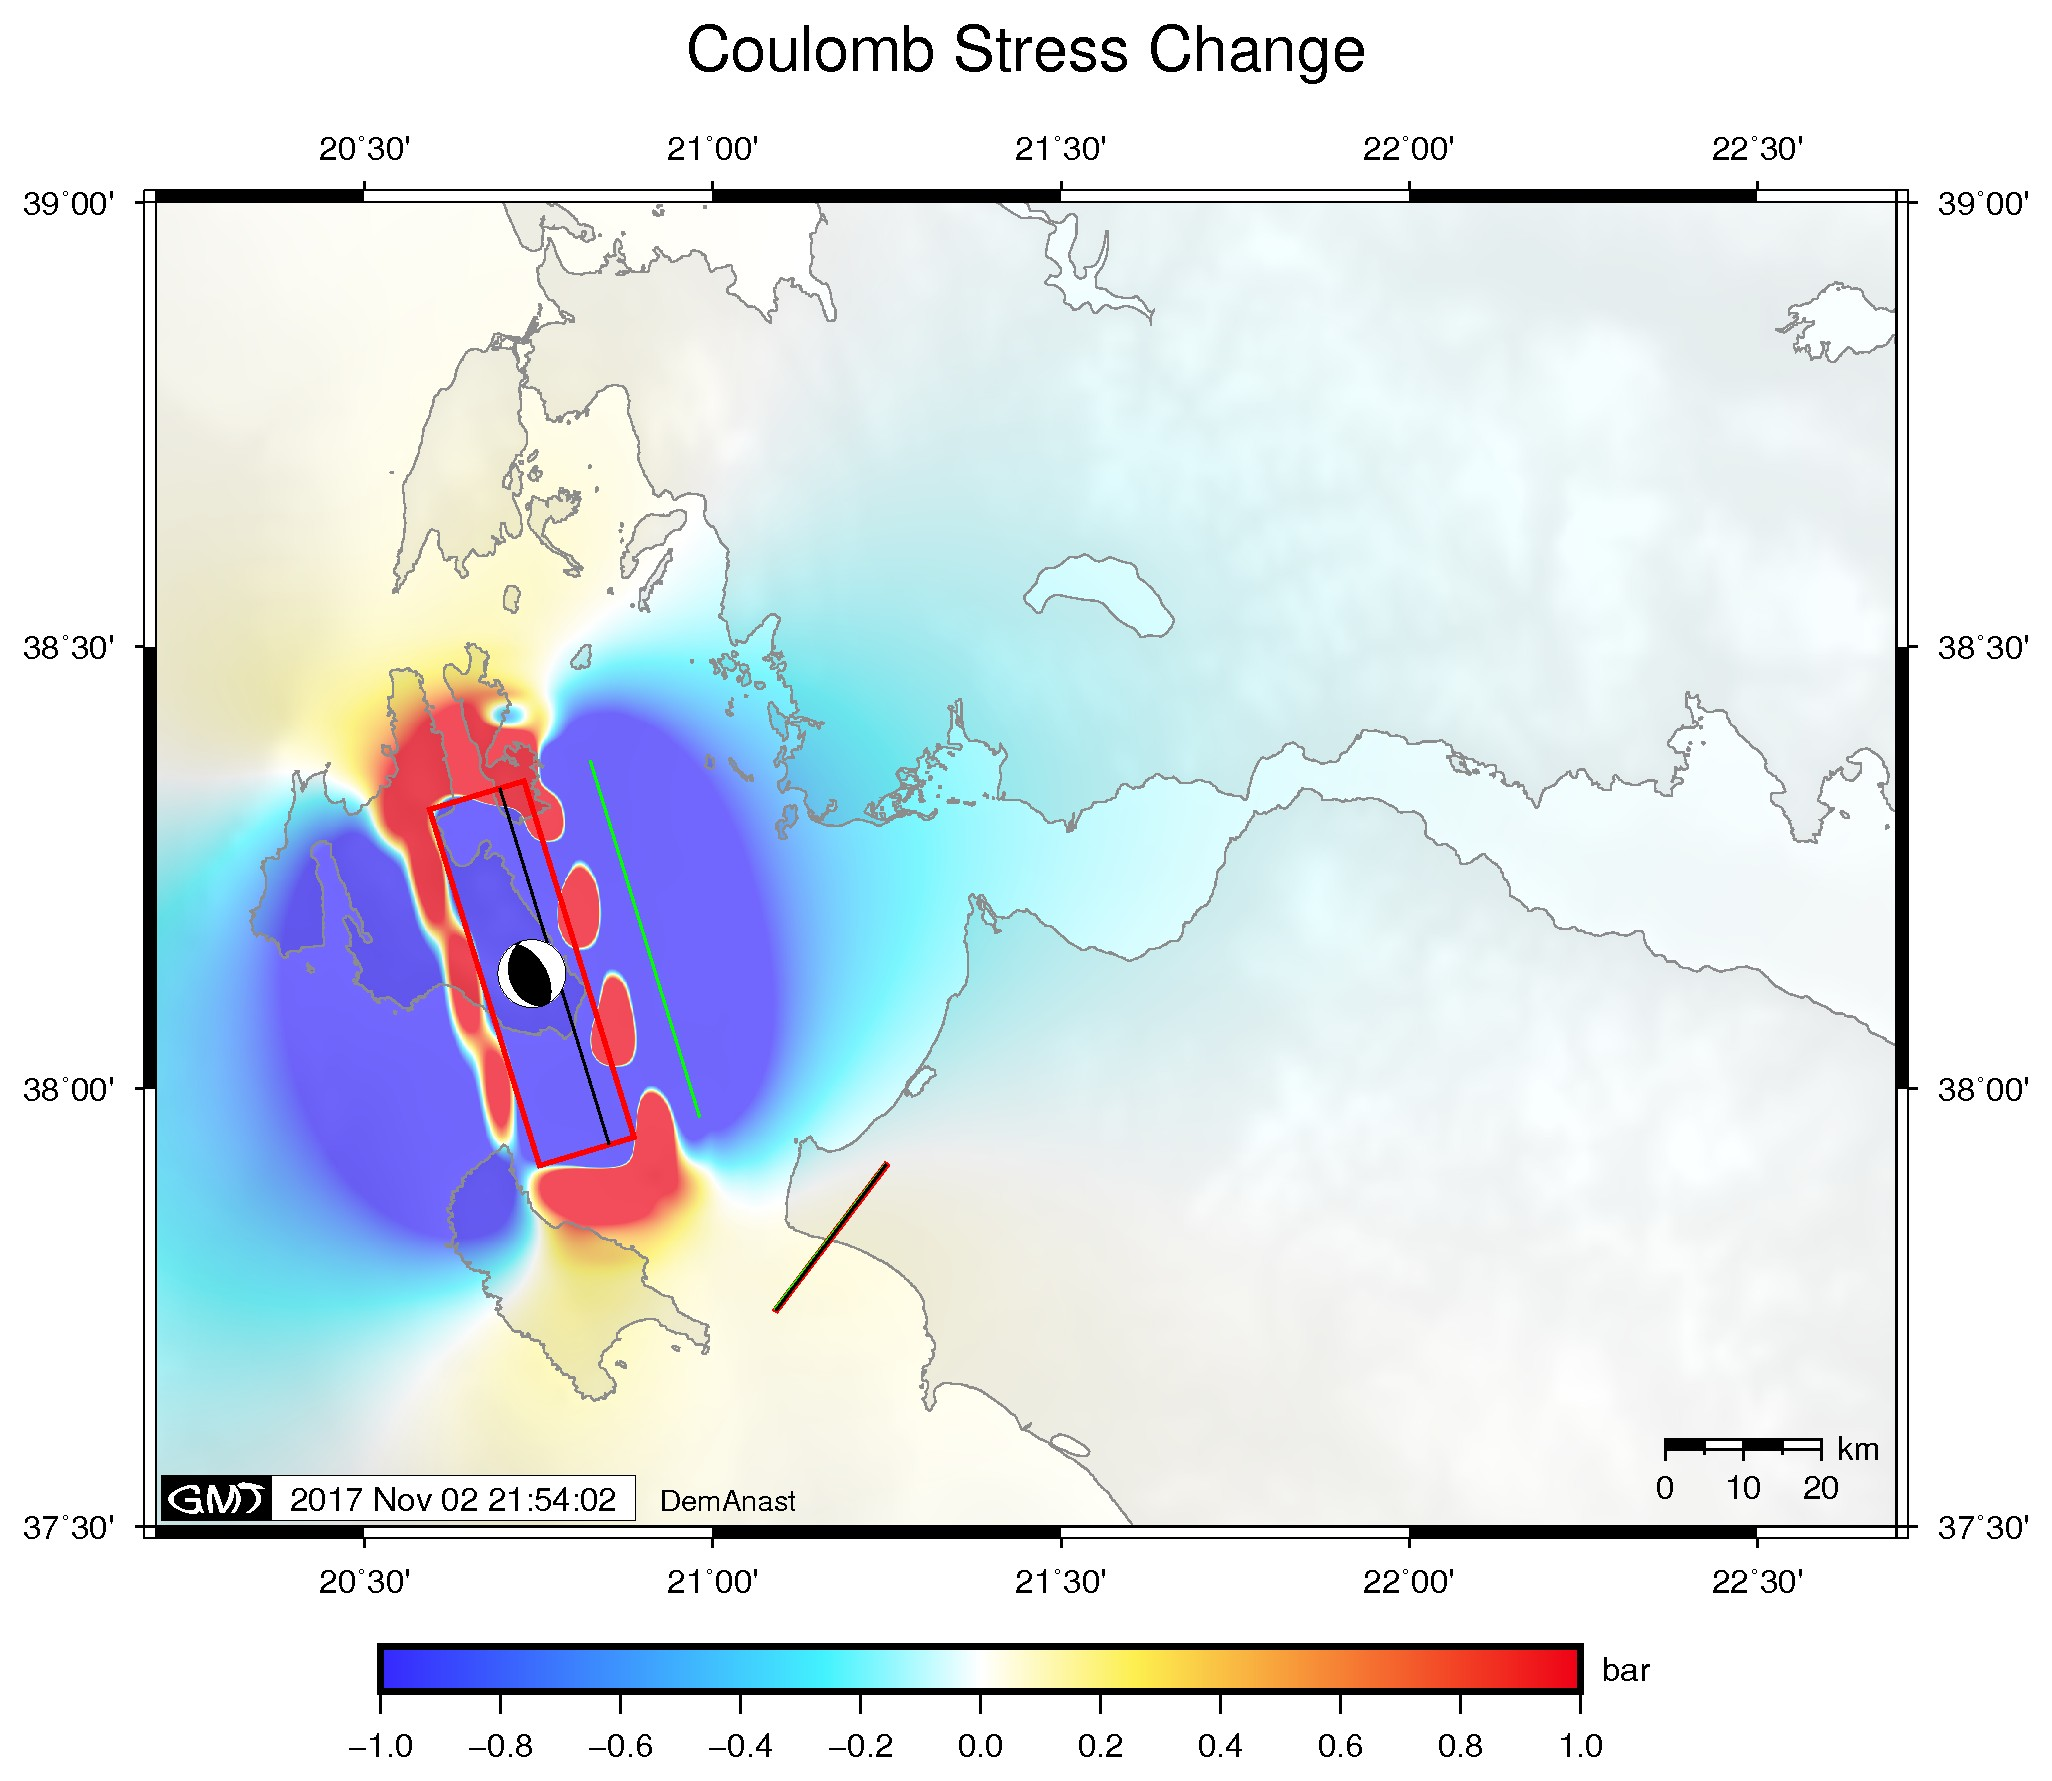
\includegraphics[width=.95\linewidth]{example502.jpg}
  \end{column}
\end{columns}

\end{frame}
\note{}

% //////////////////////////////////////////////////////////////////////////////
\begin{frame}[t,fragile]
  \frametitle{Coulomb Stress Change overlay topography and Cross Section}
  \framesubtitle{Example 503}
  \label{ch5fr:ex503}
\begin{columns}[t]
  \begin{column}{.5\textwidth}
\begin{scriptsize}
\begin{verbatim}
$ ./coulomb2gmt.sh kef_1953 kef_1953_kef \
                   -outjpg \ 
                   --output example503 \
                   --logo_gmt \
                   --moment_tensor historic.cmt \
                   -fproj \
                   -fsurf \
                   -fdep \
                   -cstress+ot \ 
                   -fcross
\end{verbatim}
\end{scriptsize}

  \end{column}
  \begin{column}{.5\textwidth}

\centering
  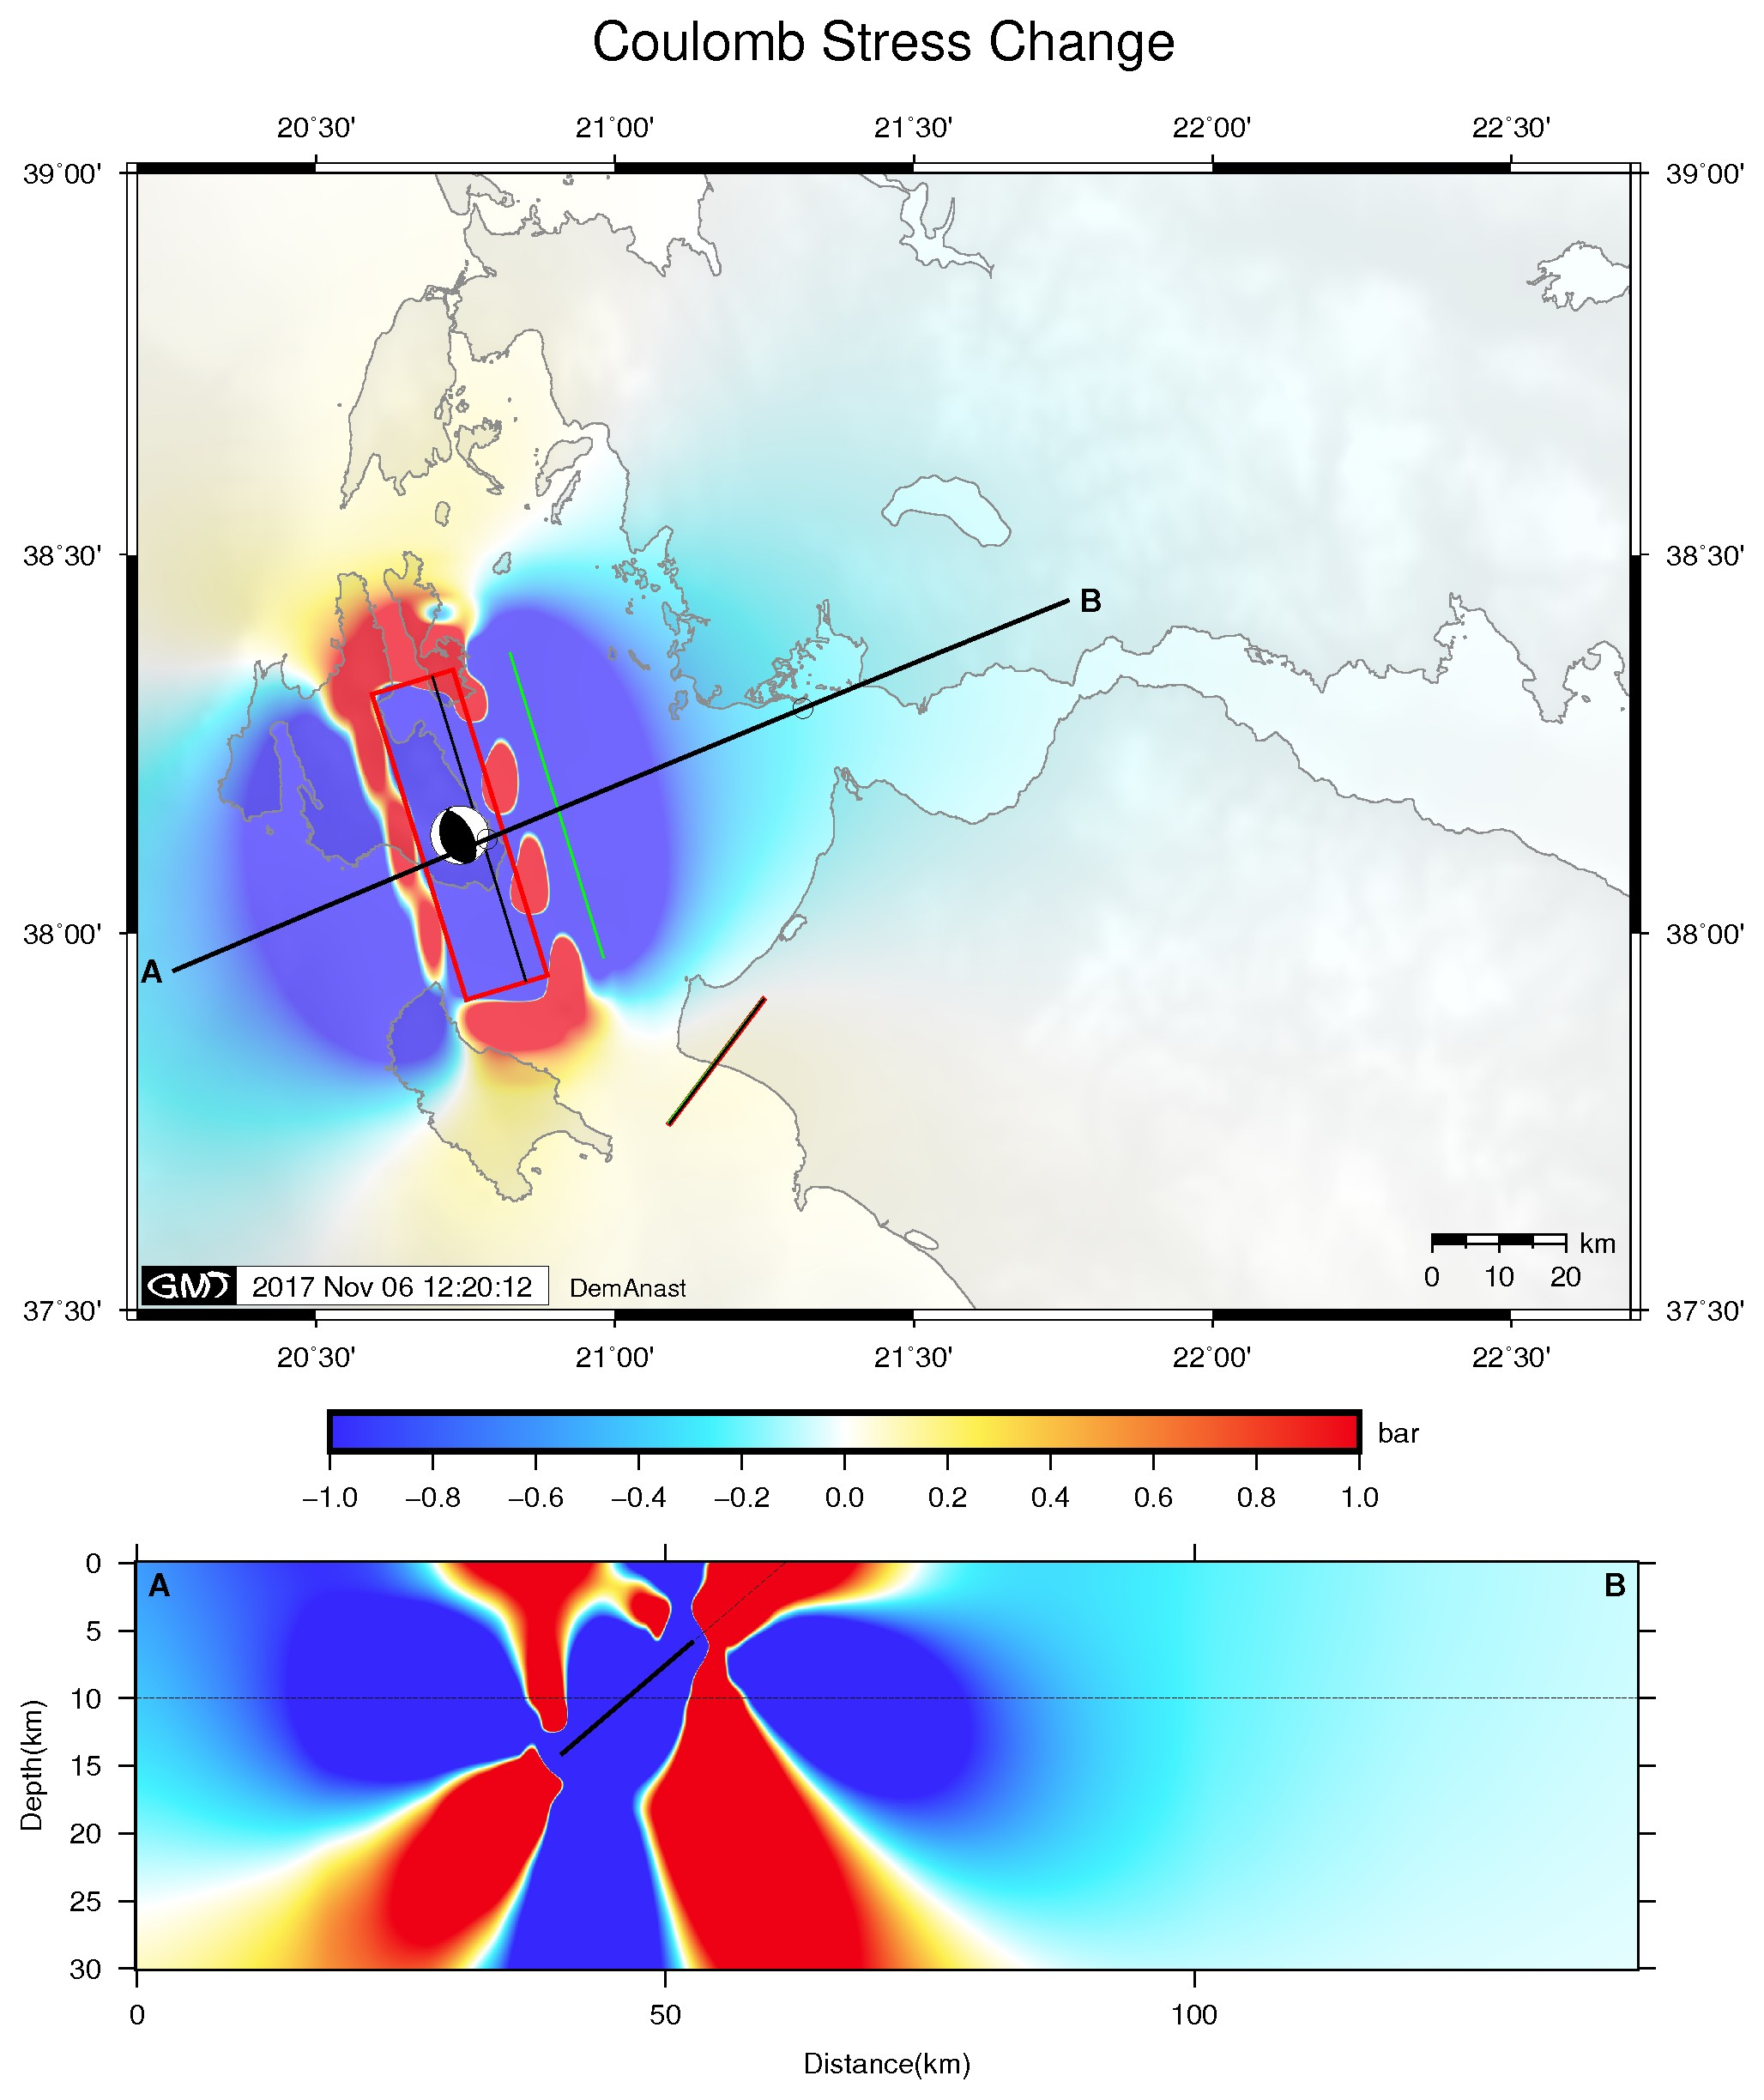
\includegraphics[width=.75\linewidth]{example503.jpg}
  \end{column}
\end{columns}

\end{frame}
\note{}

% //////////////////////////////////////////////////////////////////////////////
\begin{frame}[t,fragile]
  \frametitle{Strain Component Eyy}
  \framesubtitle{Example 504}
  \label{ch5fr:ex504}
\begin{columns}[t]
  \begin{column}{.5\textwidth}
\begin{scriptsize}
\begin{verbatim}
$ ./coulomb2gmt.sh kef_1953 kef_1953_kef \
                   -outjpg \ 
                   --output example504 \
                   --logo_gmt \
                   --moment_tensor historic.cmt \
                   -fproj \
                   -fsurf \
                   -fdep \
                   -streyy
\end{verbatim}
\end{scriptsize}

  \end{column}
  \begin{column}{.5\textwidth}

\centering
  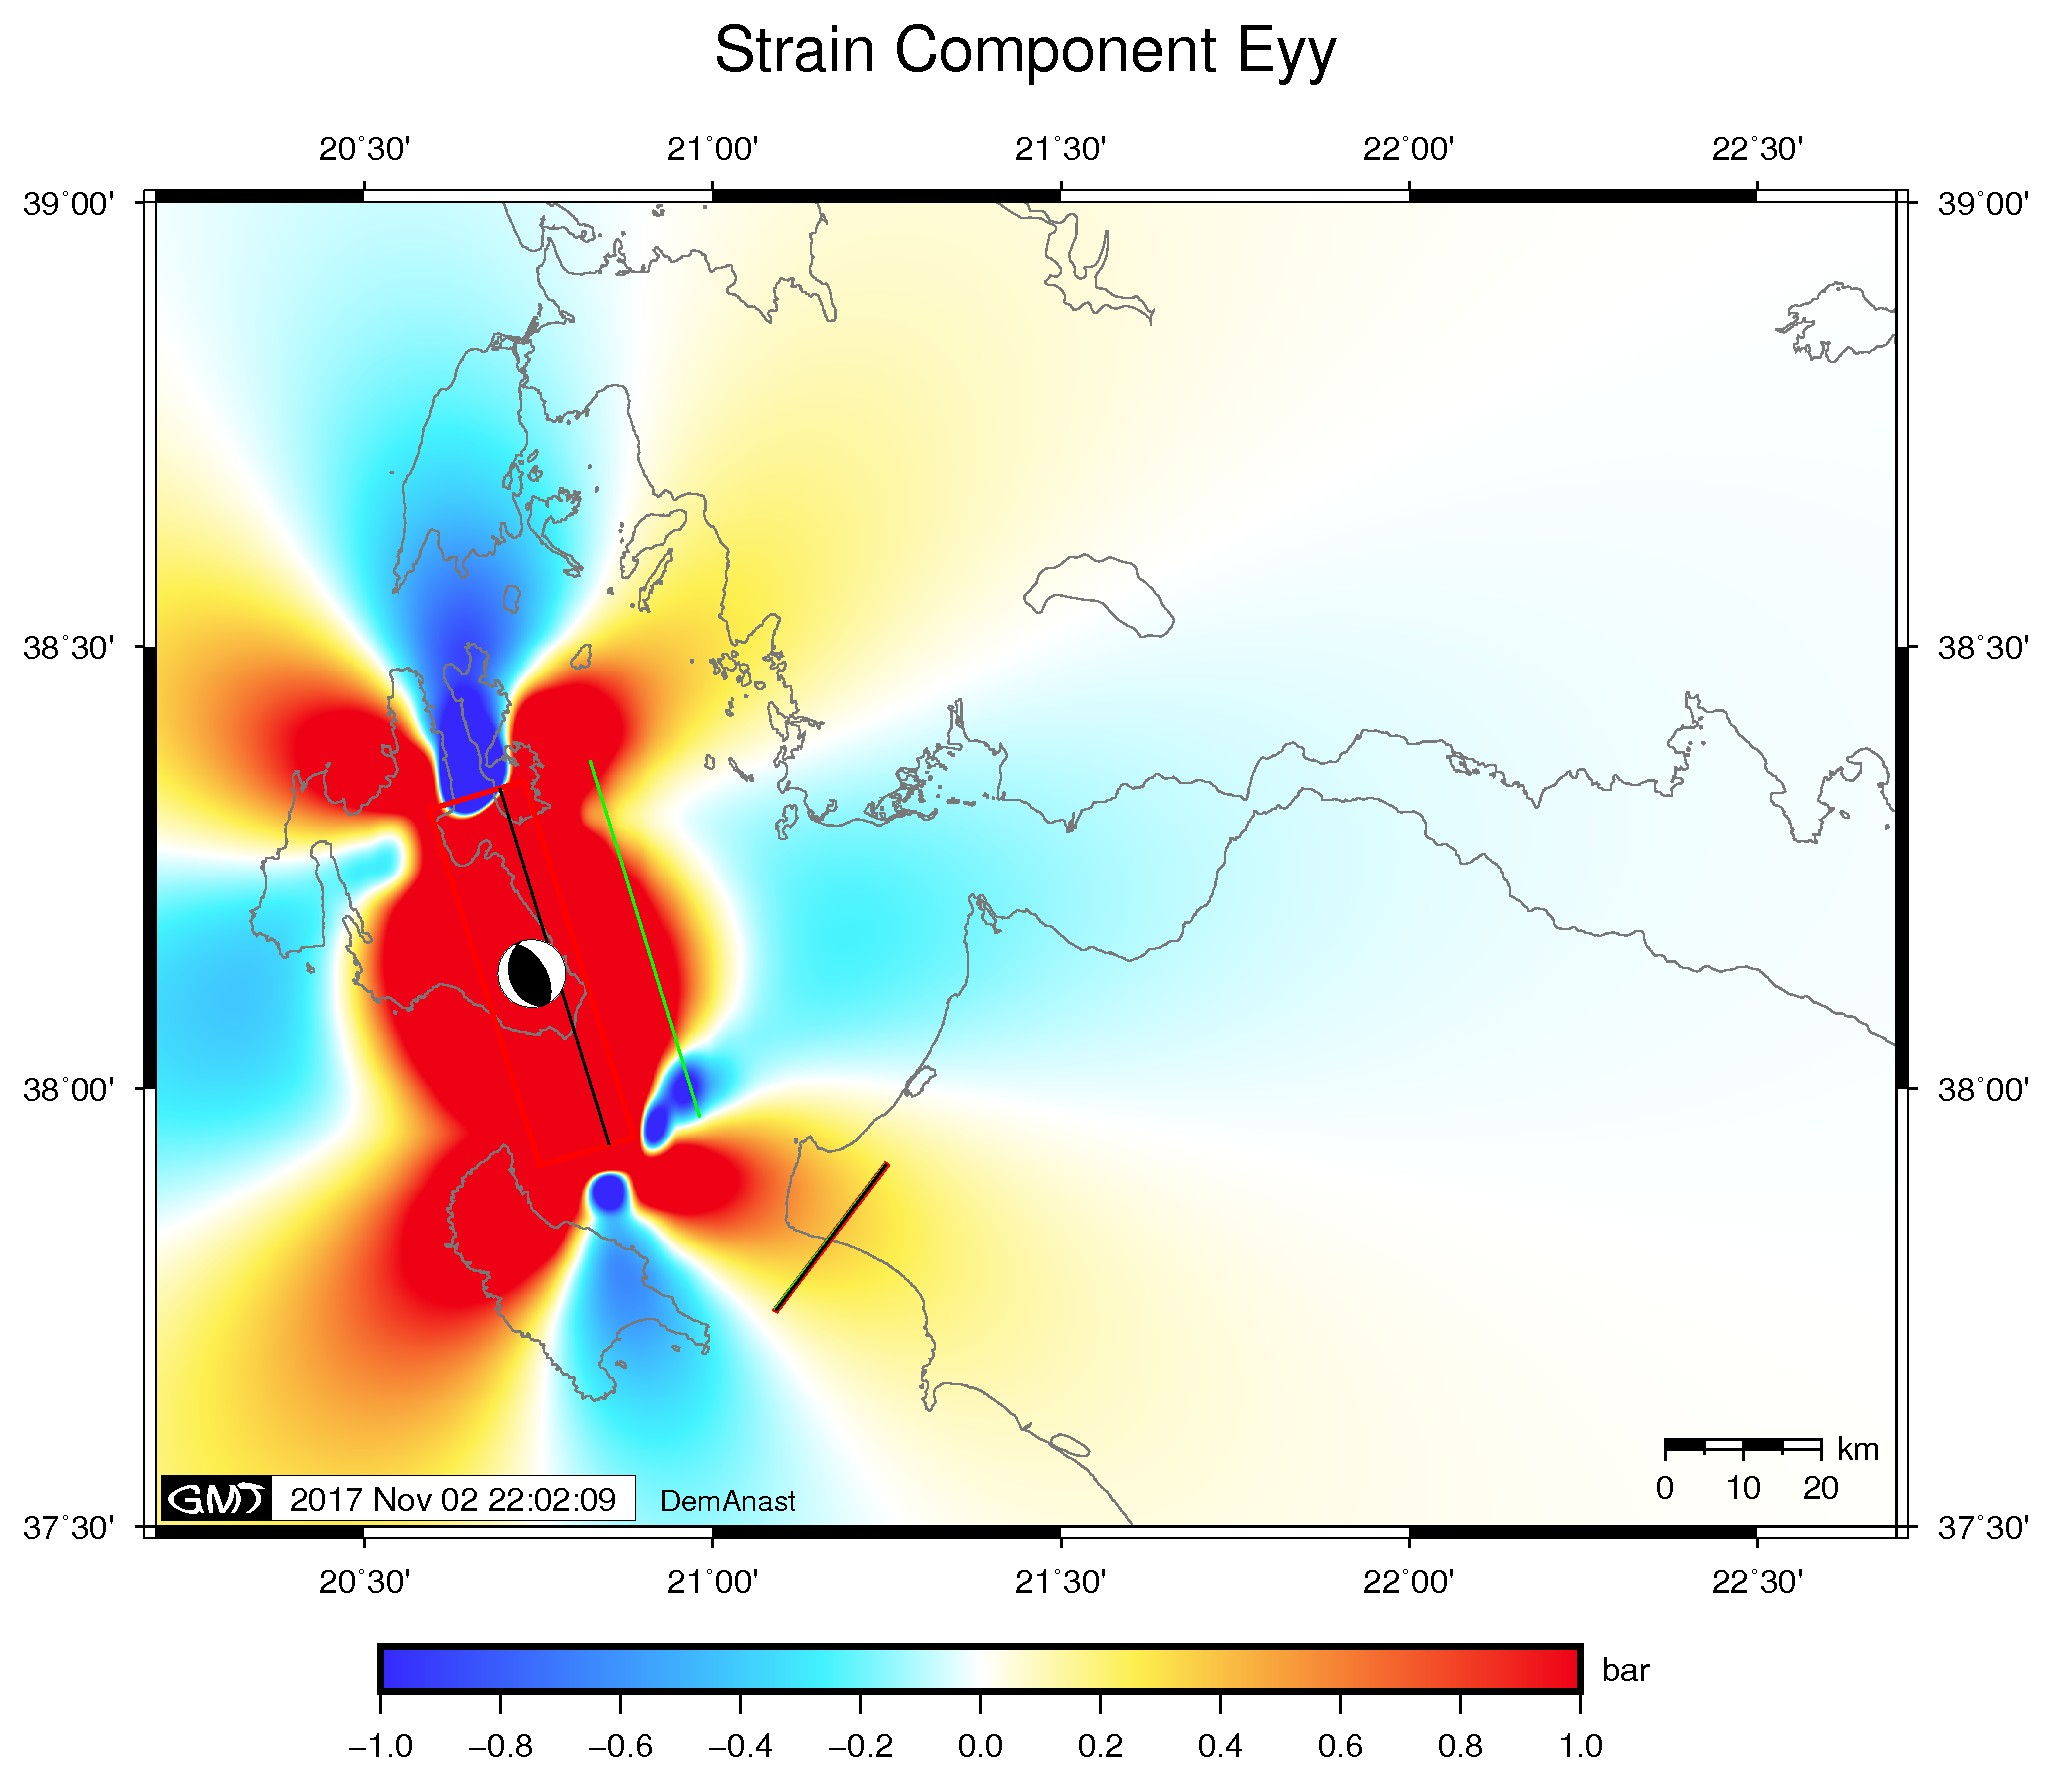
\includegraphics[width=.95\linewidth]{example504.jpg}
  \end{column}
\end{columns}

\end{frame}
\note{}

% //////////////////////////////////////////////////////////////////////////////
\begin{frame}[t,fragile]
  \frametitle{Dilatation (Exx + Eyy + Ezz) and cross section}
  \framesubtitle{Example 505}
  \label{ch5fr:ex505}
\begin{columns}[t]
  \begin{column}{.5\textwidth}
\begin{scriptsize}
\begin{verbnobox}[\vbdelim]
\$ ./coulomb2gmt.sh kef_1953 kef_1953_kef \
                   -outjpg \ 
                   --output example505 \
                   --logo_gmt \
                   --moment_tensor historic.cmt \
                   -fproj \
                   -fsurf \
                   -fdep \
                   -strdil+ot \
                   <[red]-fcross>
\end{verbnobox}
\end{scriptsize}

  \end{column}
  \begin{column}{.5\textwidth}

\centering
  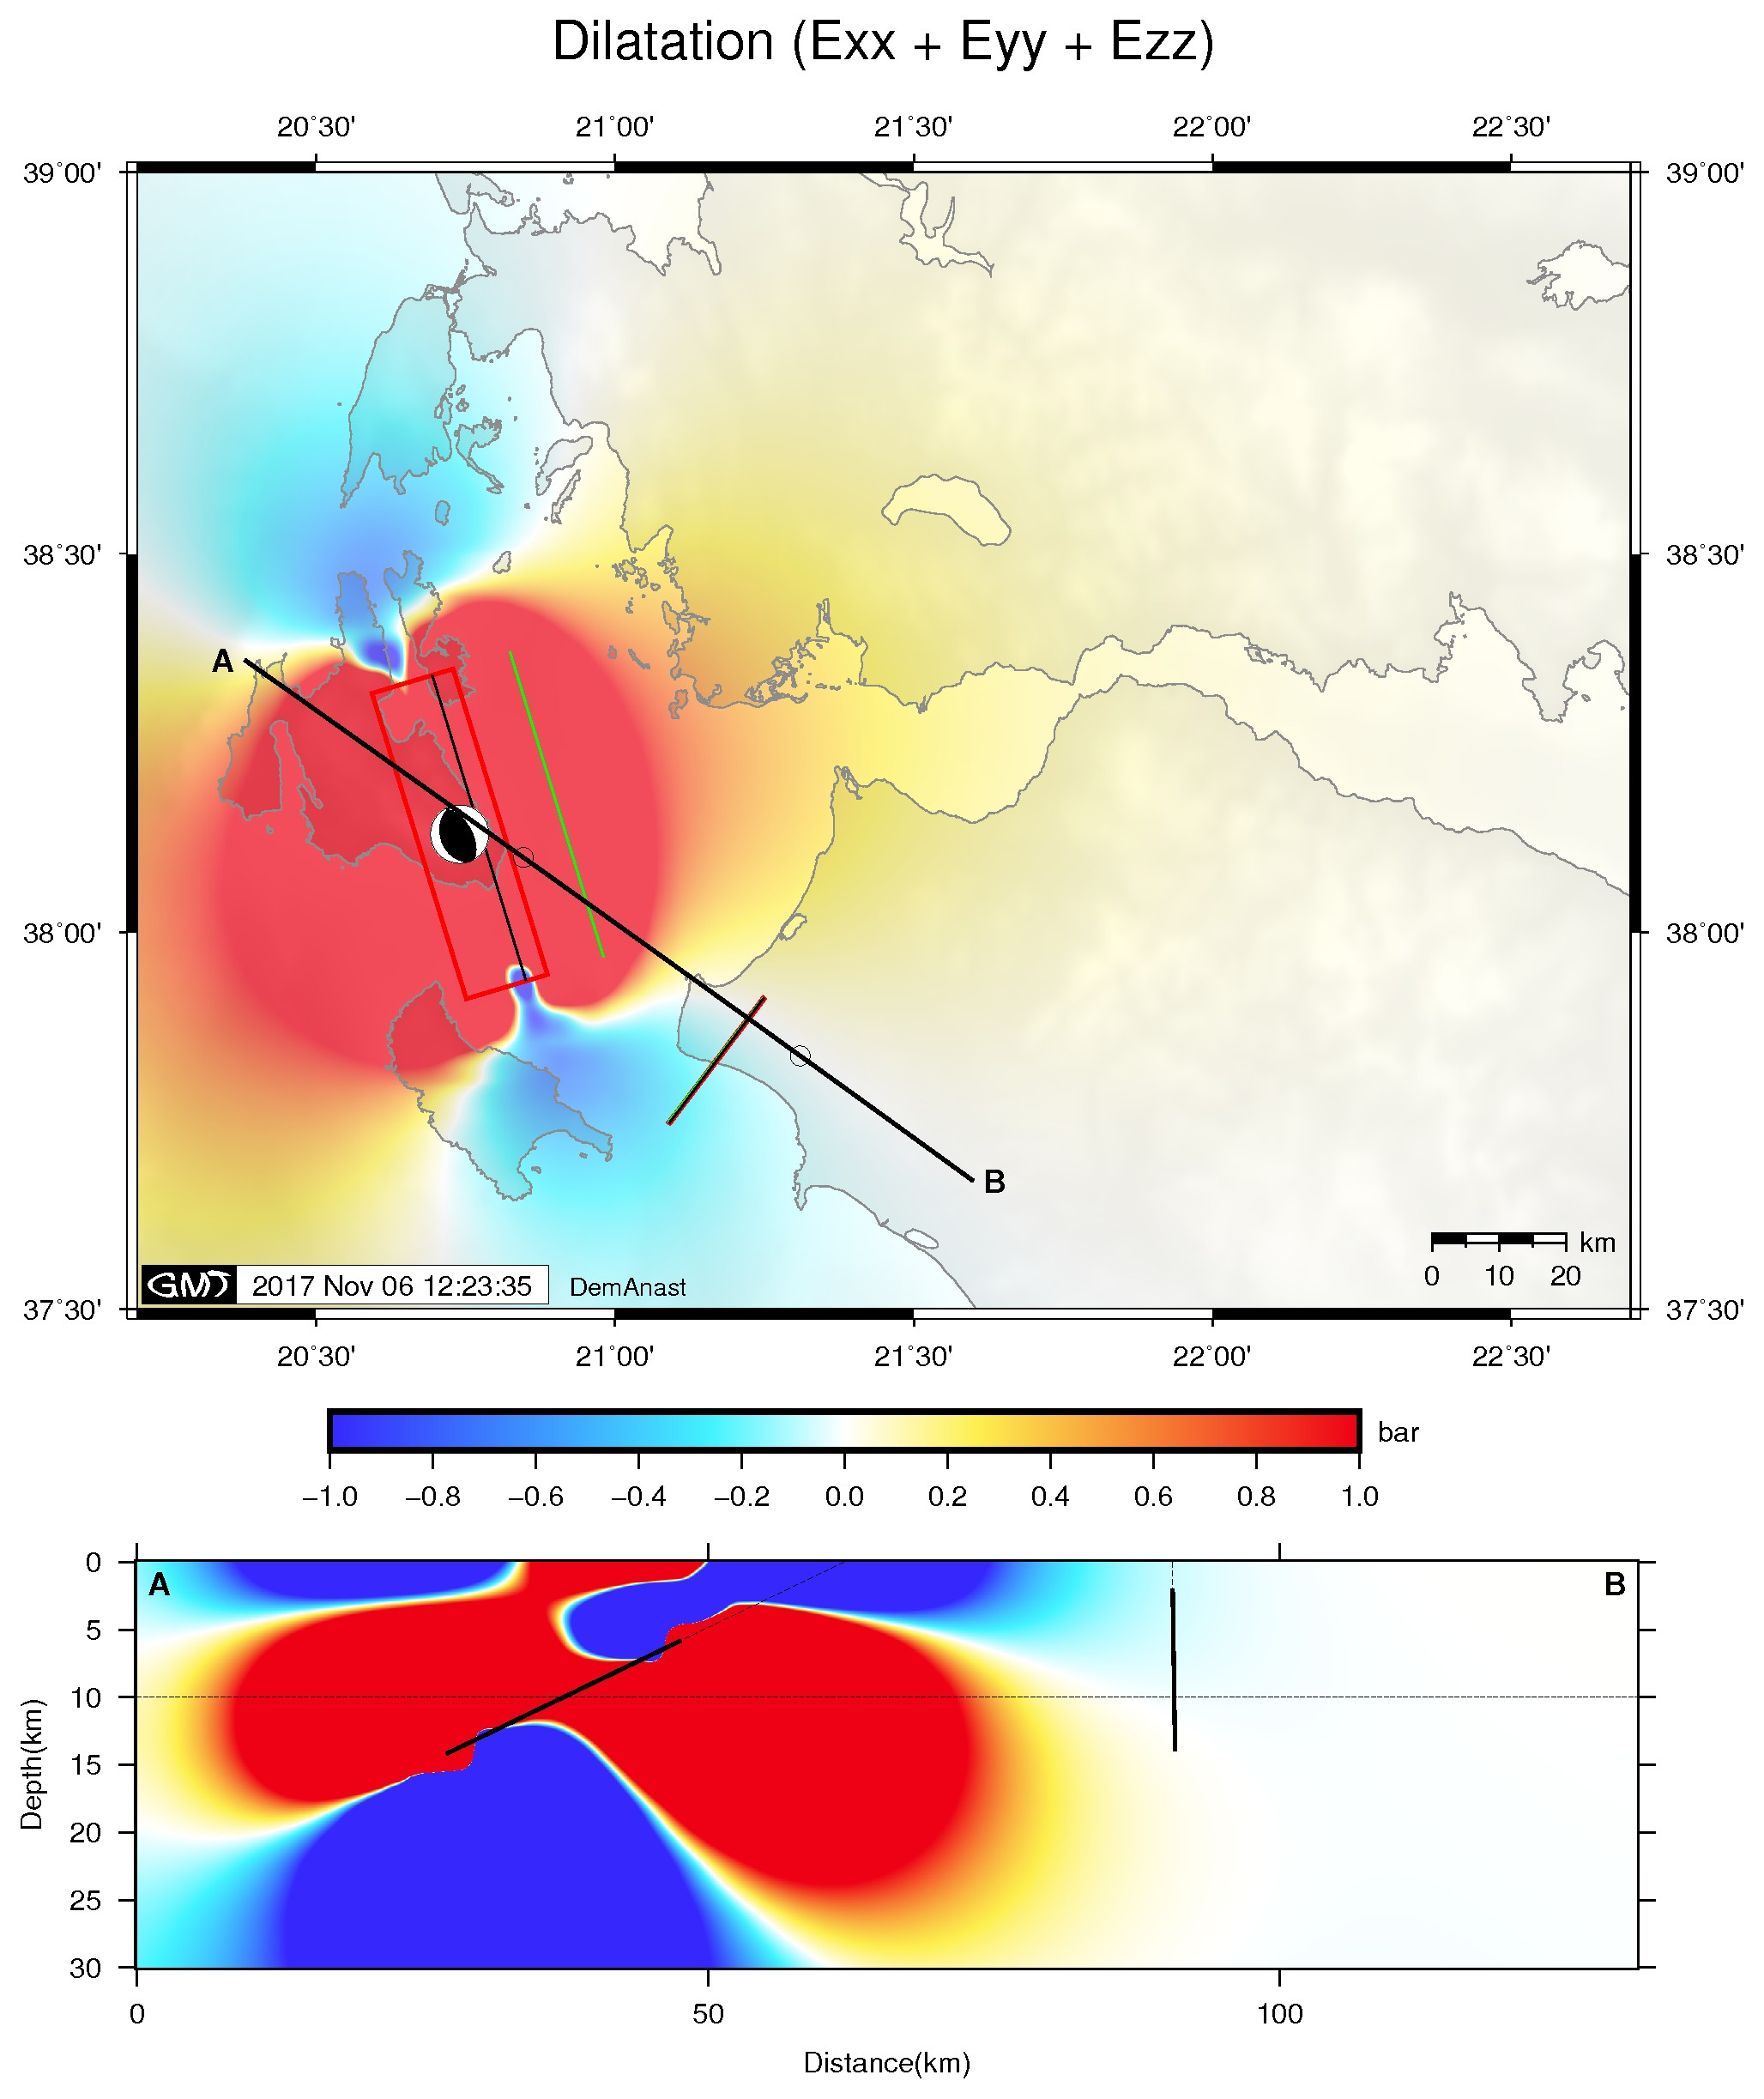
\includegraphics[width=.75\linewidth]{example505.jpg}
  \end{column}
\end{columns}

\end{frame}
\note{}




















